\section{Graftyper}
En graf er, som tidligere nævnt, en struktur med punkter og kanter. Den er givet ved definitionen:
\begin{definition}
[Graf] 
En graf $G=(V,E)$ består af $V$, en punktmængde, hvor $V\neq0$, og en kantmængde; $E \subseteq \{\{u;v\}|u,v \in V\}$.
\end{definition}
Det fremgår af definitionen, at en graf ikke kan have 0 punkter, men en lignende afgrænsning i den anden ende eksisterer ikke. Der kan altså godt være uendeligt mange knuder og kanter. I så fald kaldes det en uendelig graf. Ellers kaldes det en endelig graf, og det er denne type, som vi beskæftiger os med i projektet.
Ydermere, ses det i definitionen, at hver kant forbinder én eller to punkter. For en simpel graf gælder det, at ingen kanter forbinder et punkt med sig selv. Der må altså ikke være løkker. Derudover forbindes to punkter med max én kant.

\begin{figure}[H]
\centering
	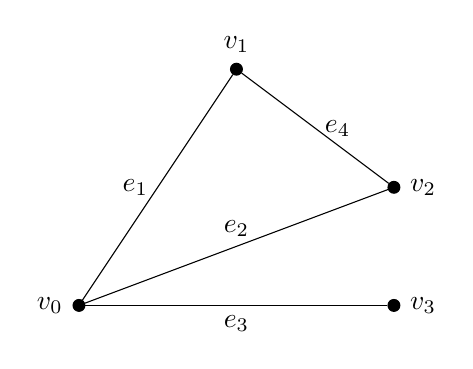
\begin{tikzpicture}

      \tikzset{enclosed/.style={draw, circle, inner sep=0pt, minimum size=.15cm, fill=black}}
%% Vertices
      	\node[enclosed, label={left: $v_0$}] (v0) at (0,0) {};
      	\node[enclosed, label={above: $v_1$}] (v1) at (2,3) {};
    	\node[enclosed, label={right: $v_2$}] (v2) at (4,1.5) {};
  	    \node[enclosed, label={right: $v_3$}] (v3) at (4,0) {};
%Edges
		\path (v0) edge node[midway, left] {$e_1$} (v1);
		\path (v0) edge node[midway, above] {$e_2$} (v2);
		\path (v0) edge node[midway, below] {$e_3$} (v3);
		\path (v1) edge node[midway, right] {$e_4$} (v2);

	\end{tikzpicture}
	\caption{En simpel graf}
	\label{fig.simpel}
\end{figure}



I kontrast til den simple graf finder vi multi-grafen. For denne type graf skal der være flere kanter, der forbinder det samme sæt punkter. Der må stadig ikke optræde løkker.

\begin{figure}[H]
\centering
	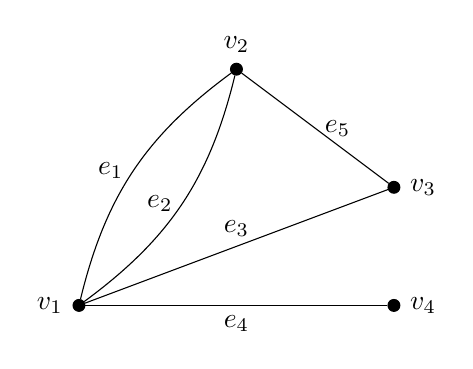
\begin{tikzpicture}

      \tikzset{enclosed/.style={draw, circle, inner sep=0pt, minimum size=.15cm, fill=black}}
%% Vertices
      	\node[enclosed, label={left: $v_1$}] (v1) at (0,0) {};
      	\node[enclosed, label={above: $v_2$}] (v2) at (2,3) {};
    	\node[enclosed, label={right: $v_3$}] (v3) at (4,1.5) {};
  	    \node[enclosed, label={right: $v_4$}] (v4) at (4,0) {};
%Edges
		\path (v1) edge [bend right=20] node[midway, left] {$e_2$} (v2);
		\path (v2) edge [bend right=20] node[midway, left] {$e_1$} (v1);
		\path (v1) edge node[midway, above] {$e_3$} (v3);
		\path (v1) edge node[midway, below] {$e_4$} (v4);
		\path (v2) edge node[midway, right] {$e_5$} (v3);

	\end{tikzpicture}
	\caption{En multigrafgraf}
	\label{fig.multi}
\end{figure}


I eksemplet ovenover ses det, at to kanter forbinder punktsættet ($v_{1},v_{2}$). Hvis en graf, modsat de to allerede nævnte, kan indeholde både løkker og flere kanter, der forbinder de samme punkter, kaldes det en pseudo-graf. Vi ser i eksemplet herunder, at der er to kanter, der forbinder $v_{1}$ og $v_{2}$, og der er en løkke ved $v_{4}$.

\begin{figure}[H]
\centering
	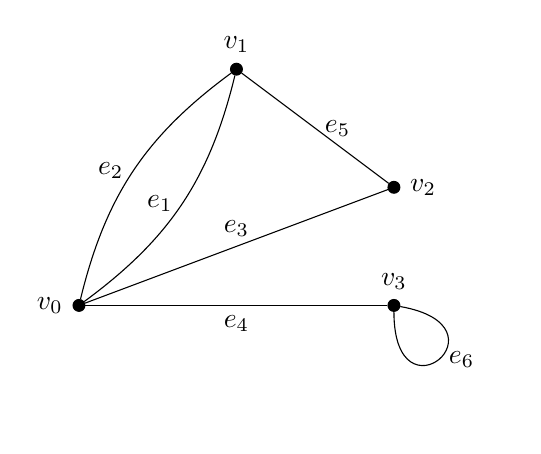
\begin{tikzpicture}[every loop/.style={}]
      \tikzset{enclosed/.style={draw, circle, inner sep=0pt, minimum size=.15cm, fill=black}}
%% Vertices
      	\node[enclosed, label={left: $v_0$}] (v0) at (0,0) {};
      	\node[enclosed, label={above: $v_1$}] (v1) at (2,3) {};
    	\node[enclosed, label={right: $v_2$}] (v2) at (4,1.5) {};
  	    \node[enclosed, label={above: $v_3$}] (v3) at (4,0) {};
%Edges
		\path (v0) edge [bend right=20] node[midway, left] {$e_1$} (v1);
		\path (v1) edge [bend right=20] node[midway, left] {$e_2$} (v0);
		\path (v0) edge node[midway, above] {$e_3$} (v2);
		\path (v0) edge node[midway, below] {$e_4$} (v3);
		\path (v1) edge node[midway, right] {$e_5$} (v2);
		\path (v3) edge [out=270,in=350,looseness=35] node[right] {$e_6$} (v3);
	\end{tikzpicture}
	\caption{En pseudograf med et loop}
	\label{fig.pseudo}
\end{figure}



\subsection{Orienterede grafer og ikke-orienterede grafer}
En anden typisk grafopdeling er opdelingen i orienterede og ikke-orienterede grafer. De grafer vi har kigget på indtil videre er ikke-orienterede grafer. For en orienteret graf gælder det, at dets kanter har en retning. Dette er ofte illustreret med pile. Den har dermed et startpunkt og et endepunkt. Disse grafer er defineret ved:

\begin{definition}
[Orienteret graf] 
En orienteret graf $(V,E)$ består af $V$, et sæt punkter(knuder), hvor $V\neq0$, og et sæt orienterede kanter, $E$. Hver orienterede kant forbinder et sæt punkter $(u,v)$, hvor $u$ er tilstødende til $v$, og $v$ er tilstødende fra $u$. Punktet $u$ kaldes begyndelsespunktet, og punktet $v$ kaldes endepunktet.
\end{definition}
\begin{figure}[H]
\centering
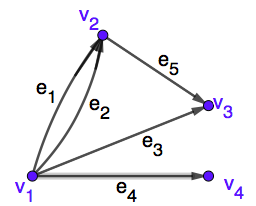
\includegraphics[scale=0.5]{fig/img/orienteret_graf.png}
\caption{En orienteret graf}
\label{fig:orienteret}
\end{figure}
Der kan foruden disse to også være tale om mixede grafer, som er grafer med både orienterede og ikke-orienterede kanter. Orienterede grafer kan ligesom ikke-orienterede grafer indeholde loops og flere kanter der forbinder det samme punktsæt. Den må også indeholde to modsatrettede kanter mellem det samme punktpar. Dvs. en kant må gerne gå fra $v$ til $u$, selvom en anden kant går fra $u$ til $v$. Hvis en orienteret graf hverken indeholder loops eller flere kanter, der forbinder det samme punktpar, kaldes den en orienteret simpel graf. Hvis der derimod optræder flere kanter mellem et eller flere punktpar, kaldes det en multigraf.Vi kan se egenskaberne for de forskellige grafer herunder:

\begin{tabular}{ |p{4cm}||p{3cm}|p{3cm}|p{2cm}|  }
 \hline
 \multicolumn{4}{|c|}{Grafer} \\
 \hline
 Type & Kanter & Flere Kanter pr punktpar tilladt? & Løkker tilladt\\
 \hline
 Simpel graf   & Ikke-orienteret    & Nej &   Nej\\
 Multigraf &   Ikke-orienteret & Ja   & Nej\\
 Pseudograf & Ikke-orienteret & Ja &  Ja\\
 Simpel orienteret graf    & Orienteret & Nej &  Nej\\
 Orienteret multigraf &  Orienteret  & Ja & Ja\\
 Mixet graf & Ikke-orienteret og orienteret  & Ja   & Ja\\
 \hline
\end{tabular}

Fordi kanterne i grafer med orienterede kanter er ordnede par kan definitionen af punktets grader være antallet af kanter, der har dette punkt som begyndelsespunkt, eller antallet af kanter, der har dette punkt som endepunkt:
\begin{definition}
[Graden af en orienteret graf] 
I en graf med orienterede kanter er ind-graden, betegnet ved $deg^{-}(v)$, antallet af kanter med v som deres endepunkt. Ud-graden, betegnet ved $deg^{+}(v)$, er antallet af kanter med v som deres startpunkt.
\end{definition}
Vi vil i projektet beskæftige os med orienterede grafer, da det er denne type vi bruger til optimeringen af gaslageret. I vores tilfælde vil vi tildele vores orienterede kanter vægt, hvilket beskrives senere i projektet.
